\section{استخراج رابطه با استفاده از مولد بازنمایی مشترک و شبکه‌های عصبی پیچشی کوتاه‌مدت بلند تکه‌ای \cite{lstm-pcnn}}

در این مقاله که در سال ۲۰۱۸ توسط دانفنگ یان\LTRfootnote{DANFENG YAN} و بو هو\LTRfootnote{BO HU} عرضه شده است،
از یک شبکه عصبی مولد برای ایجاد بازنمایی‌ رابطه استفاده شده است. این شبکه مولد برای ایجاد بازنمایی رابطه از بازنمایی جملات
آن رابطه کمک می‌گیرد. بازنمایی جمله نیز با استفاده از
شبکه‌های عصبی پیچشی کوتاه‌مدت بلند تکه‌ای\LTRfootnote{Piecewise-LSTM Convolutional Neural Network} انجام می‌شود.

\subsection{شبکه‌های عصبی کد‌گذار}

در روش‌های ارائه شده پیش از این مقاله، کدگذاری خام ارائه شده توسط \lr{PCNN} در قسمت‌های بعدی برای تعیین
رابطه بیان شده در جمله استفاده می‌شد. در این مقاله اما پس از کدگذاری جمله توسط شبکه \lr{PCNN} این کدگذاری‌ها مطابق
شکل \ref{pcnn_lstm} به یک شبکه \lr{BiLSTM} داده می‌شود تا ارتباط موجود بین قسمت‌های مختلف جمله در بازنمایی ارائه شده نهایی
تاثیرگذار باشد. کدگذاری تولید شده توسط این شبکه در شبکه‌ مولد که در بخش بعدی خواهیم دید، به کار گرفته می‌شود.

\begin{figure}[h]
    \centering
    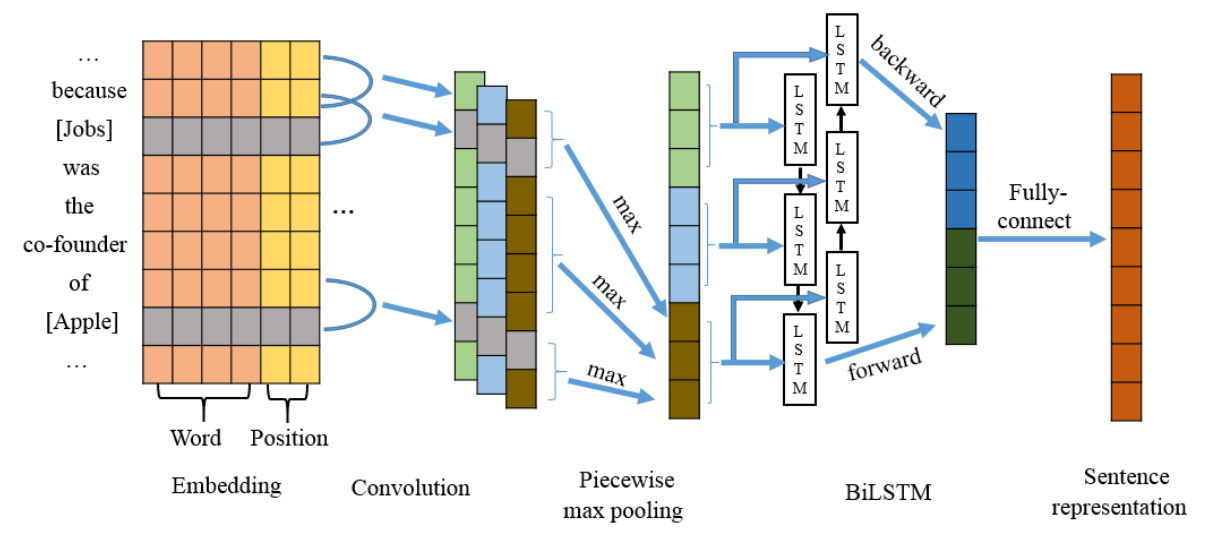
\includegraphics[width=0.8\linewidth]{images/shared/encoder.png}
    \caption{ترکیب شبکه عصبی \lr{PCNN} و \lr{LSTM}}
    \label{pcnn_lstm}
\end{figure}

\subsection{شبکه تولید‌کننده بازنمایی مشترک}

یان و هو شبکه عصبی موجود در شکل \ref{shared_representation_generator_network} را برای ایجاد بازنمایی یک دسته\LTRfootnote{bag}
از کلمات ارائه کردند. آن‌ها بر خلاف پژوهش‌های دیگر به جای آن که از مجموع وزن‌دار بازنمایی هر جمله ($s_{(i,r)}$) برای تولید
بازنمایی مشترک استفاده کنند، پیشنهاد یک مولد برای تولید بازنمایی جملات یک رابطه را مطرح کردند. این مدل مولد برای تولید
بازنمایی رابطه از بازنمایی تولید شده برای جملات متناظر رابطه استفاده می‌کند. برای آموزش این شبکه تابع خطایی نیز
معرفی شده است که ترکیبی از تابع خطای آنتروپی متقابل\LTRfootnote{cross entropy} و میانگین فاصله است.
در ادامه با جزئیات بیشتر این شبکه عصبی و تابع خطای معرفی شده آشنا می‌شویم.

شبکه عصبی مولد برای ایجاد بازنمایی رابطه از بازنمایی‌های جمله‌ که توسط مدل کدگذار \lr{PCNN} تولید شده استفاده می‌کند.
بازنمایی جمله ارائه شده توسط شبکه \lr{PCNN} به شبکه عصبی دولایه داده می‌شود. شبکه عصبی دولایه بازنمایی جمله $i$ام در رابطه
$r$ام را از فضای $s_{(i,r)}$ به فضای $g_{(i,r)}$ می‌برد. هدف از این تبدیل ایجاد یک بازنمایی بهتر با تاکید بیشتر روی معنا از بازنمایی
جمله است. در مدل پیشنهادی آن‌ها برای هر رابطه شبکه مولد جداگانه‌ای در نظر گرفته شده است که از شبکه مولد دیگر
مستقل است.

\begin{figure}[h]
    \centering
    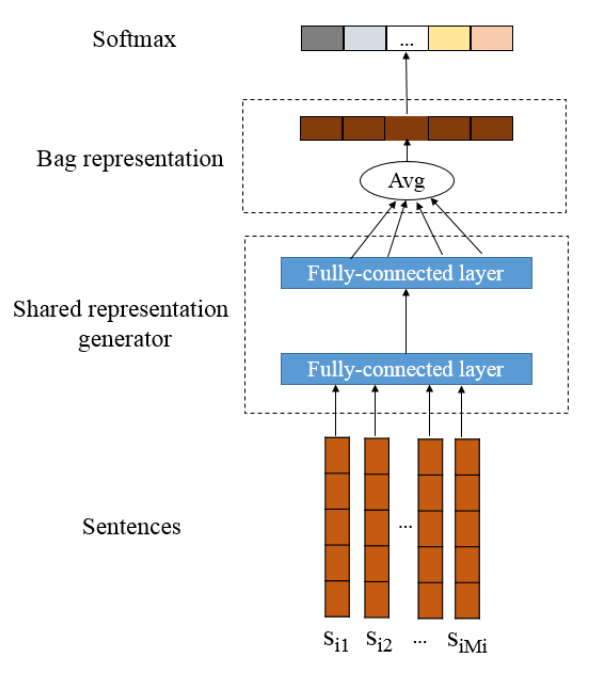
\includegraphics[scale=0.4]{images/shared/shared_repre.png}
    \caption{شبکه عصبی تولید‌کننده بازنمایی مشترک}
    \label{shared_representation_generator_network}
\end{figure}

پس از ایجاد بردار‌های $g_{(i,r)}$، میانگین بدون وزن این بردار‌ها محاسبه می‌شود. بردار حاصل شده $G_{r}$
را بردار بازنمایی آن رابطه می‌نامند.

$$G_{r} = \frac{1}{M} \sum_{i=1}^{M} g_{(i,r)}$$

از آن‌جا که آموزش مدل روی نمونه‌ها به صورت دسته‌ای بوده است، بنابراین در هنگام آزمایش مدل داده‌ها به صورت
دسته‌ای به مدل مولد داده شده و رابطه کلی بیان شده توسط آن‌ دسته با استفاده از یک لایه بیشینه‌گیری نرم\LTRfootnote{softmax}
مشخص می‌شود.

حال که جزئیات شبکه مولد بیان شد، جزئیات تابع خطای متناظر آن تشریح می‌شود. تابع خطای این شبکه دو هدف را دنبال می‌کند:

\begin{enumerate}
    \item بازنمایی ارائه شده برای یک رابطه تا جای امکان دور از بازنمایی رابطه‌های دیگر باشد.
    \item بازنمایی ارائه شده تا جای امکان مشابه بازنمایی ارائه شده برای هر جمله آن رابطه باشد.
\end{enumerate}

برای رسیدن به هدف اول، از تابع خطای آنتروپی متقابل استفاده می‌شود. بدین ترتیب که انتظار می‌رود لایه بیشینه‌گیری‌ نرم
بتواند برچسب دسته را به درستی تعیین کند. به عبارت ریاضی حاصل عبارت زیر باید بیشینه شود.

\begin{eqnarray}
    J_1(\theta) = \sum_{i=1}^{T} \log p(r_i|G_i,\theta)
\end{eqnarray}

برای رسیدن به هدف دوم نیاز است که فاصله بازنمایی تولید شده از هر جمله متناظر آن رابطه کمینه باشد. برای رسیدن
به این هدف تابع خطای $J_2(\theta)$ به صورت زیر محاسبه می‌شود.

\begin{eqnarray}
    J_2(\theta) & = & \frac{1}{T} \sum_{i=1}^{T} (\frac{1}{M_i} \sum_{j=1}^{M_i} (g_{(j,i)} - c_i)^2) \\
    c_i & = & \frac{1}{M_i} \sum_{j=1}^{M_i} g_{(j,i)}
\end{eqnarray}

نکته عجیبی که در تابع خطای بالا وجود دارد استفاده از بازنمایی $g_{(i,r)}$ به جای $s_{(i,r)}$ است. چرا که
$G_r$ میانگین \textbf{بدون وزن} از $g_{(i,r)}$ است بنابراین محاسبه فاصله آن تا هر یک از $g_{(i,r)}$ به نظر نمی‌رسد که
پارامتری را تحت تاثیر قرار دهد. اما اگر این مقدار از روی $s_{(i,r)}$ از روی محاسبه می‌شد با توجه به این که $g_{(i,r)}$
از یک شبکه عصبی محاسبه می‌شود بنابراین پارامتر‌های این شبکه را تحت تاثیر قرار می‌داد.

در نهایت تابع خطای کل به صورت زیر محاسبه می‌شود.

\begin{eqnarray}
    J(\theta) = J_1(\theta) + \alpha J_2(\theta)
\end{eqnarray}
